\label{chapter-5}

\section{Infrastructure used}

Eth2dgraph was developed and used on a server provided by the Decentralised Systems Engineering Lab of the NTNU University. The server's specifications are reported in \cref{table:server-specs}.

\begin{table}[ht!]
\centering
    \begin{threeparttable}
    \begin{tabular}  { m{3cm} m{6cm} } 
    \toprule
    \textbf{Parameter} & \textbf{Value}   \\
    \midrule
    CPU    &    64 cores, 256 threads \\[1.3ex]
    RAM    &    1.5 TB \\[1.3ex]
    OS    &     Ubuntu 22.04 \\[1.3ex]
    Disk    &   16 TB SSD array \\[1.3ex]
    \bottomrule
    \end{tabular}
    \end{threeparttable}
\caption[Specification of the server used for the work]{Specification of the server used for the work.}
\label{table:server-specs}
\end{table}

On this same machine there was an archive Ethereum node that was used to get the data. The RPC calls did not have to go trough the network, all the process was done in a single machine. The client used was Erigon\footnote{Erigon is an Ethereum client written in Go \url{https://github.com/ledgerwatch/erigon}}. It was run with the command reported in \cref{lst:erigon-command} and the RPC daemon with the command reported in \cref{lst:rpc-command}.

\begin{lstlisting}[language=bash,caption={Erigon command},label={lst:erigon-command},captionpos=b,numbers=none]
erigon \
    --datadir="our data location" \
    --chain=mainnet \
    --authrpc.jwtsecret="JWT secret location"\
    --private.api.addr=0.0.0.0:9090 \
    --http.api=eth,debug,net,trace,web3,erigon
\end{lstlisting}

\begin{lstlisting}[language=bash,caption={RPC daemon command},label={lst:rpc-command},captionpos=b,numbers=none]
rpcdaemon \
    --datadir="our data location" \
    --http.addr=0.0.0.0 \
    --http.api=eth,debug,net,trace,web3,erigon
\end{lstlisting}

\subsection{Benchmark of the Erigon's RPC interface}

To give a clearer overview of the environment in which data extraction was done, I performed a load test against the Erigon node using a modified version of \textit{flood}\footnote{Flood is an open-source tool for load testing Ethereum nodes \url{https://github.com/paradigmxyz/flood}}. I tested the throughput and the success rate, varying the requests per second, of the three RPCs used by eth2dgraph: {\tt eth\_getBlockByNumber}, {\tt eth\_getLogs} and {\tt trace\_block}. Flood was modified to generate RPC calls with the exact same parameters used by eth2dgraph, spread over random block numbers. The actual network calls were performed by \textit{vegeta}\footnote{Vegeta is a tool written in Go for load testing HTTP services \url{https://github.com/tsenart/vegeta}}, that is specifically designed to measure HTTP services with a constant request rate. Each load test was conducted for 30 seconds. \cref{fig:logs-success,fig:logs-throughput,fig:blocks-success,fig:blocks-throughput,fig:traces-success,fig:traces-throughput}~show the results of this test. The slowest RPC, and so the bottleneck of data extraction, resulted to be {\tt trace\_block}. 

% LOGS
\begin{figure}[H]
    \centering
    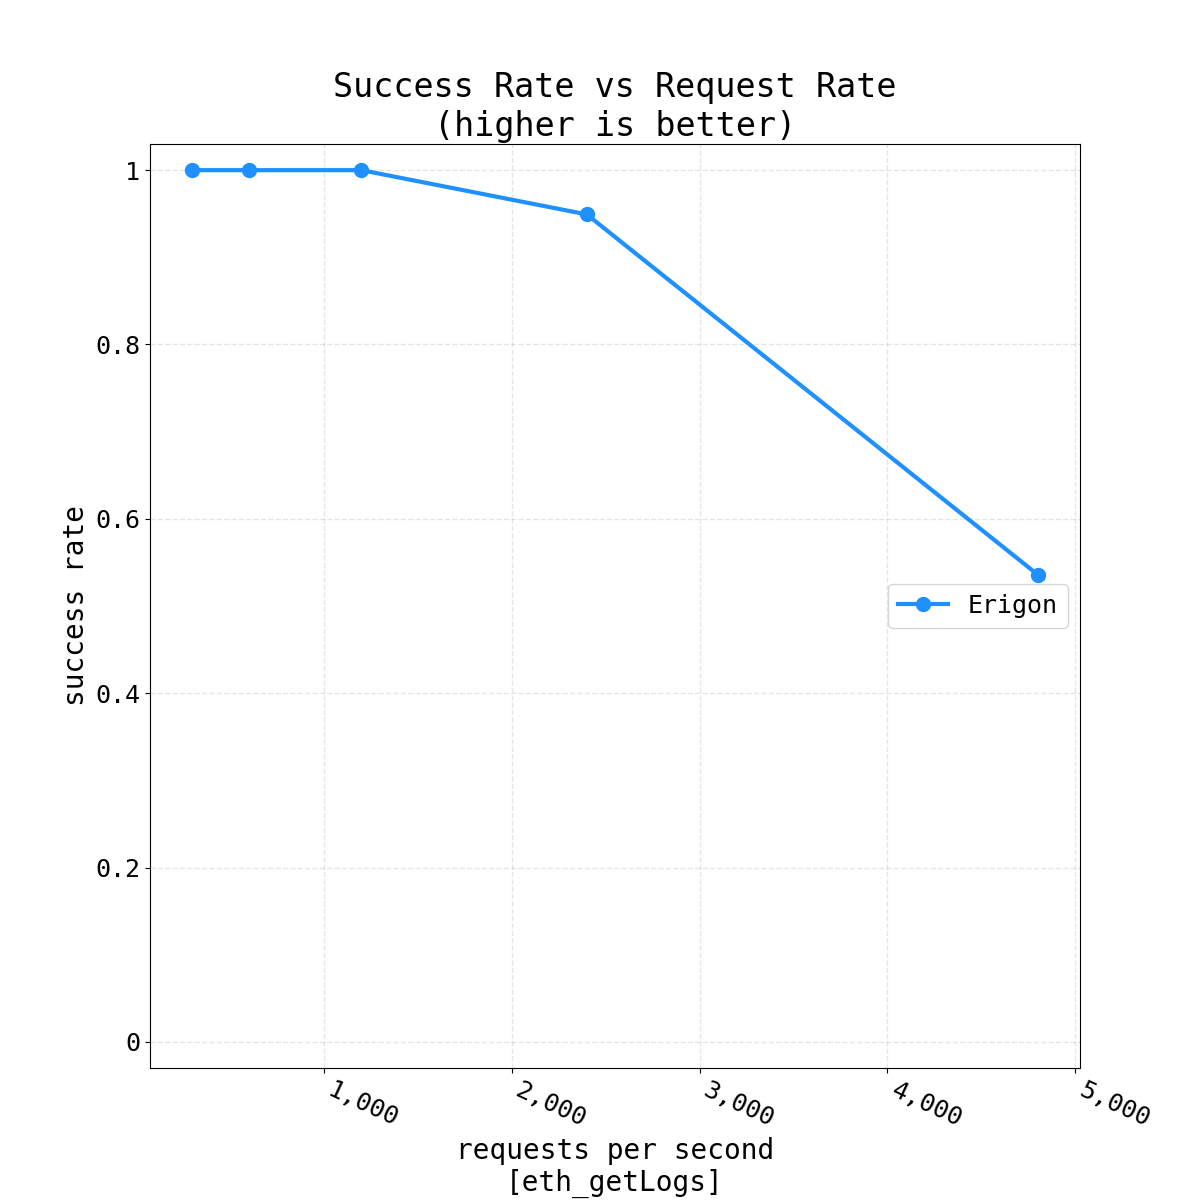
\includegraphics[width=0.7\textwidth]{Figures/results/load_tests/logs/success_rate_logs.png}
    \caption{Success rate of {\tt eth\_getLogs}. After 1200 requests/s, Erigon starts to fail handling some requests. At 5k requests/s half of the requets fail. }
    \label{fig:logs-success}
\end{figure}

\begin{figure}[H]
    \centering
    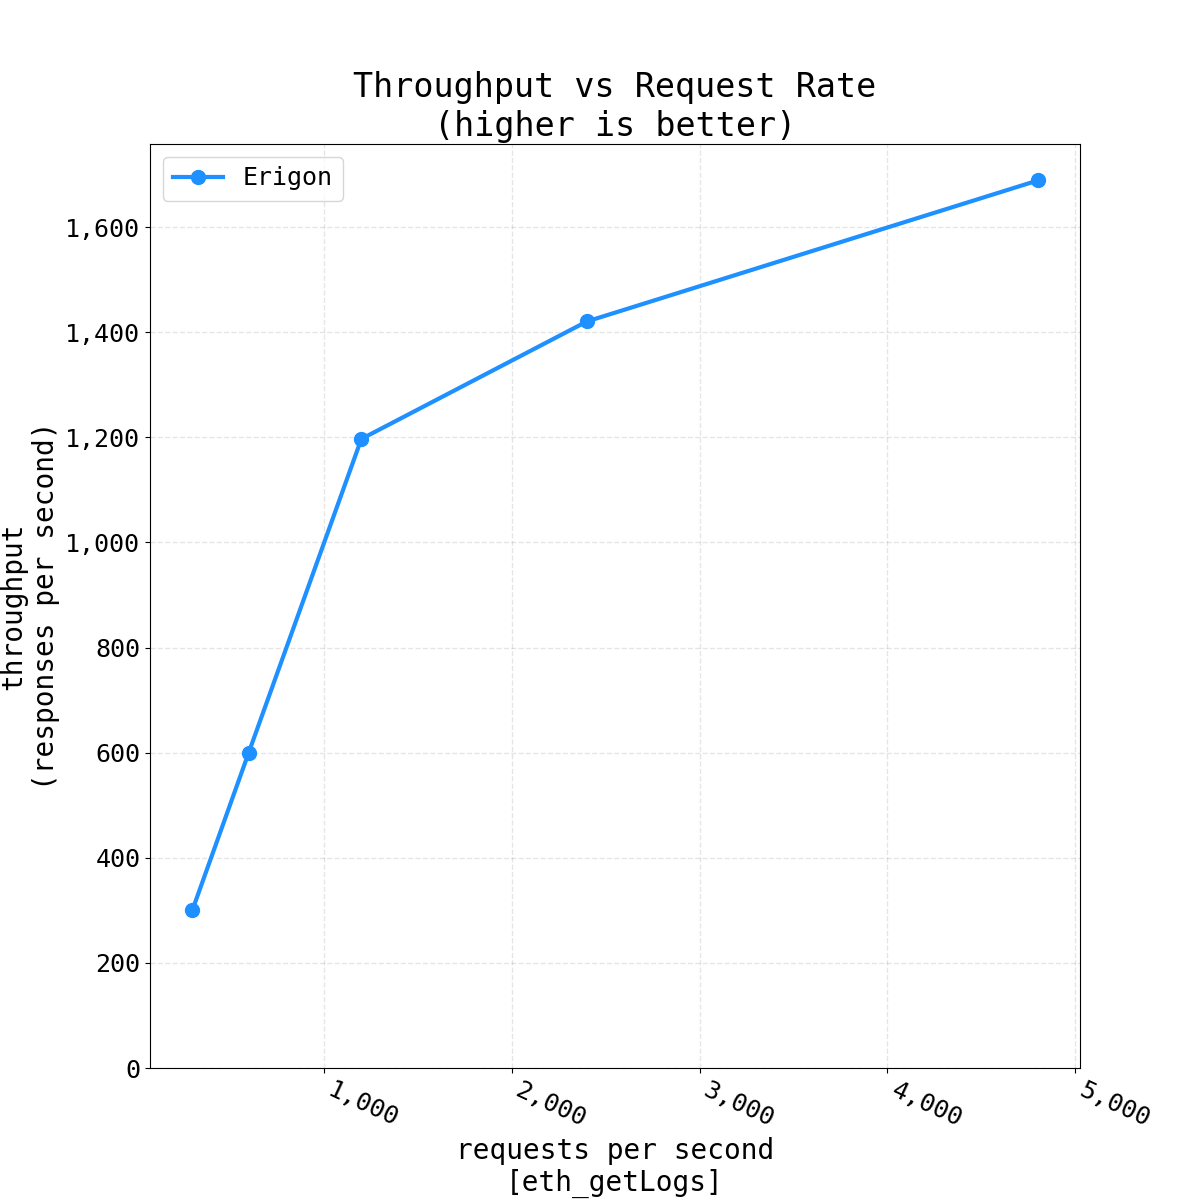
\includegraphics[width=0.7\textwidth]{Figures/results/load_tests/logs/throughput_logs.png}
    \caption{Throughput of {\tt eth\_getLogs}. After 1200 requests/s Erigon can't keep the requests rate. }
    \label{fig:logs-throughput}
\end{figure}

% BLOCKS    
\begin{figure}[H]
    \centering
    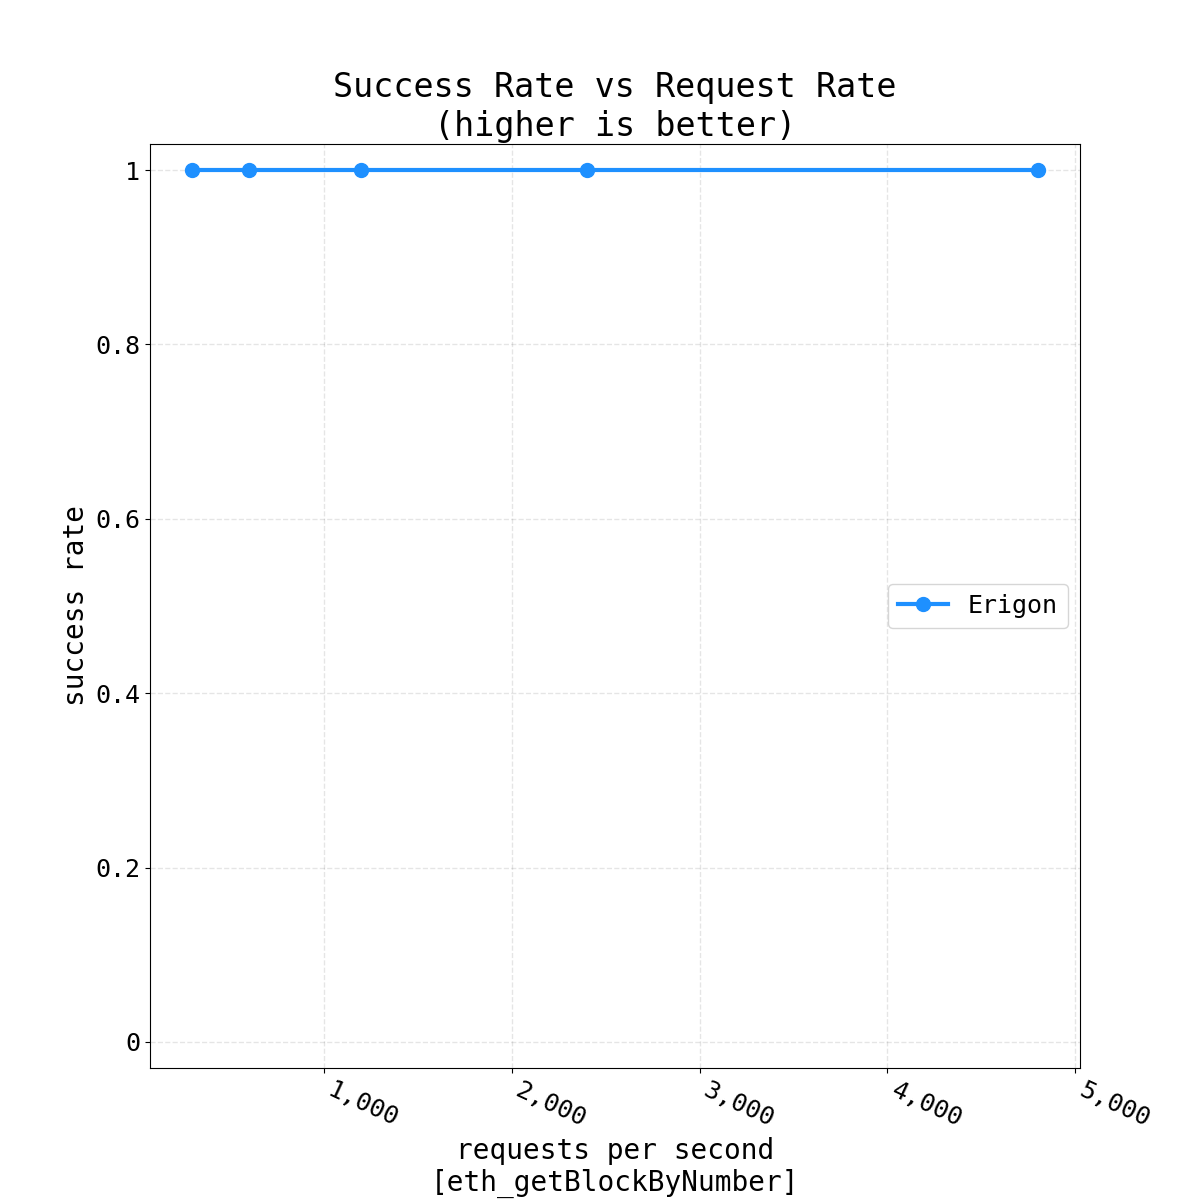
\includegraphics[width=0.7\textwidth]{Figures/results/load_tests/blocks/success_rate_blocks.png}
    \caption{Success rate of {\tt eth\_getBlockByNumber}. Erigon shows perfect performance on this RPC. It can succesfully reply to 5k requests/s. }
    \label{fig:blocks-success}
\end{figure}

\begin{figure}[H]
    \centering
    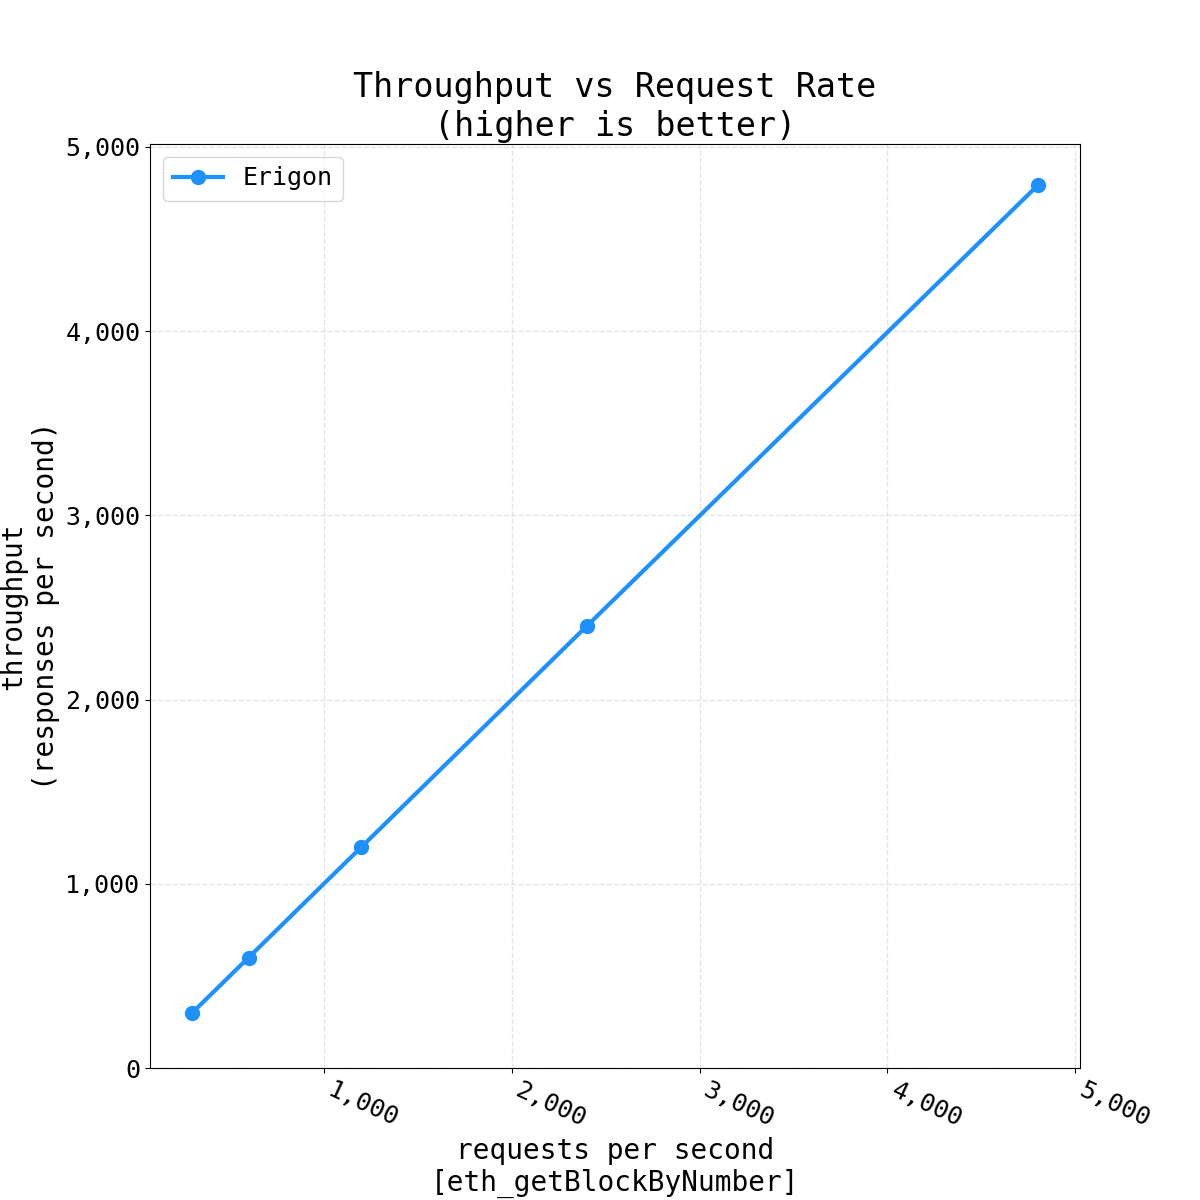
\includegraphics[width=0.7\textwidth]{Figures/results/load_tests/blocks/throughput_blocks.png}
    \caption{Throughput of {\tt eth\_getBlockByNumber}. Erigon can keep the throughput even at 5k requests/s.  }
    \label{fig:blocks-throughput}
\end{figure}

% TRACES    
\begin{figure}[H]
    \centering
    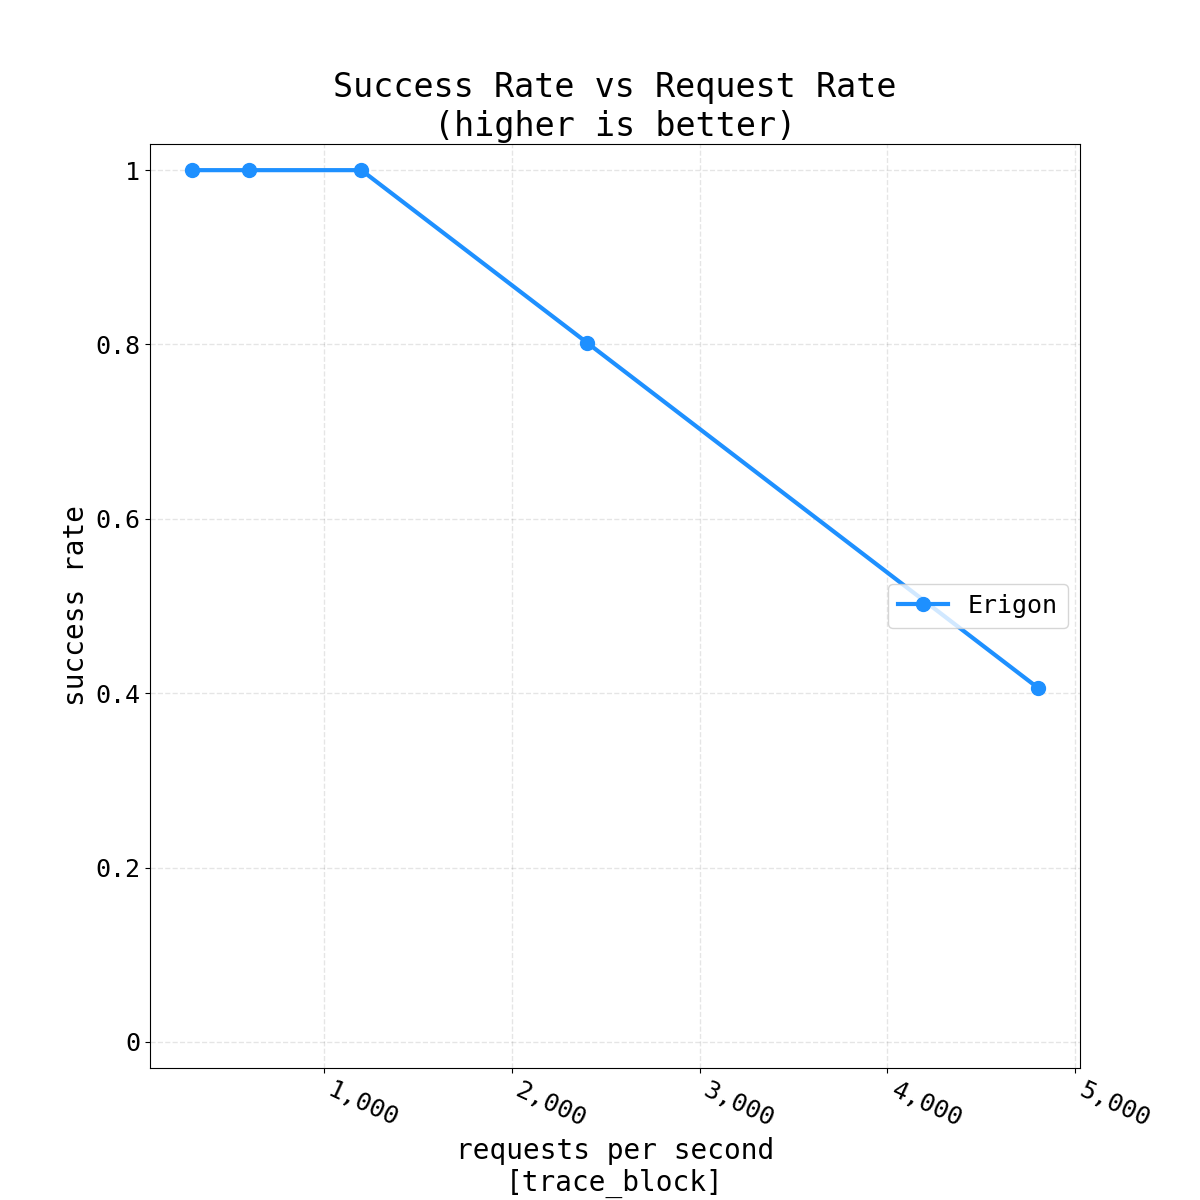
\includegraphics[width=0.7\textwidth]{Figures/results/load_tests/traces/success_rate_trace.png}
    \caption{Success rate of {\tt trace\_block}. Erigon starts to degrade after 1200 requests/s. At 5k requests/s, just 40\% of the requests are successfully handled.  }
    \label{fig:traces-success}
\end{figure}

\begin{figure}[H]
    \centering
    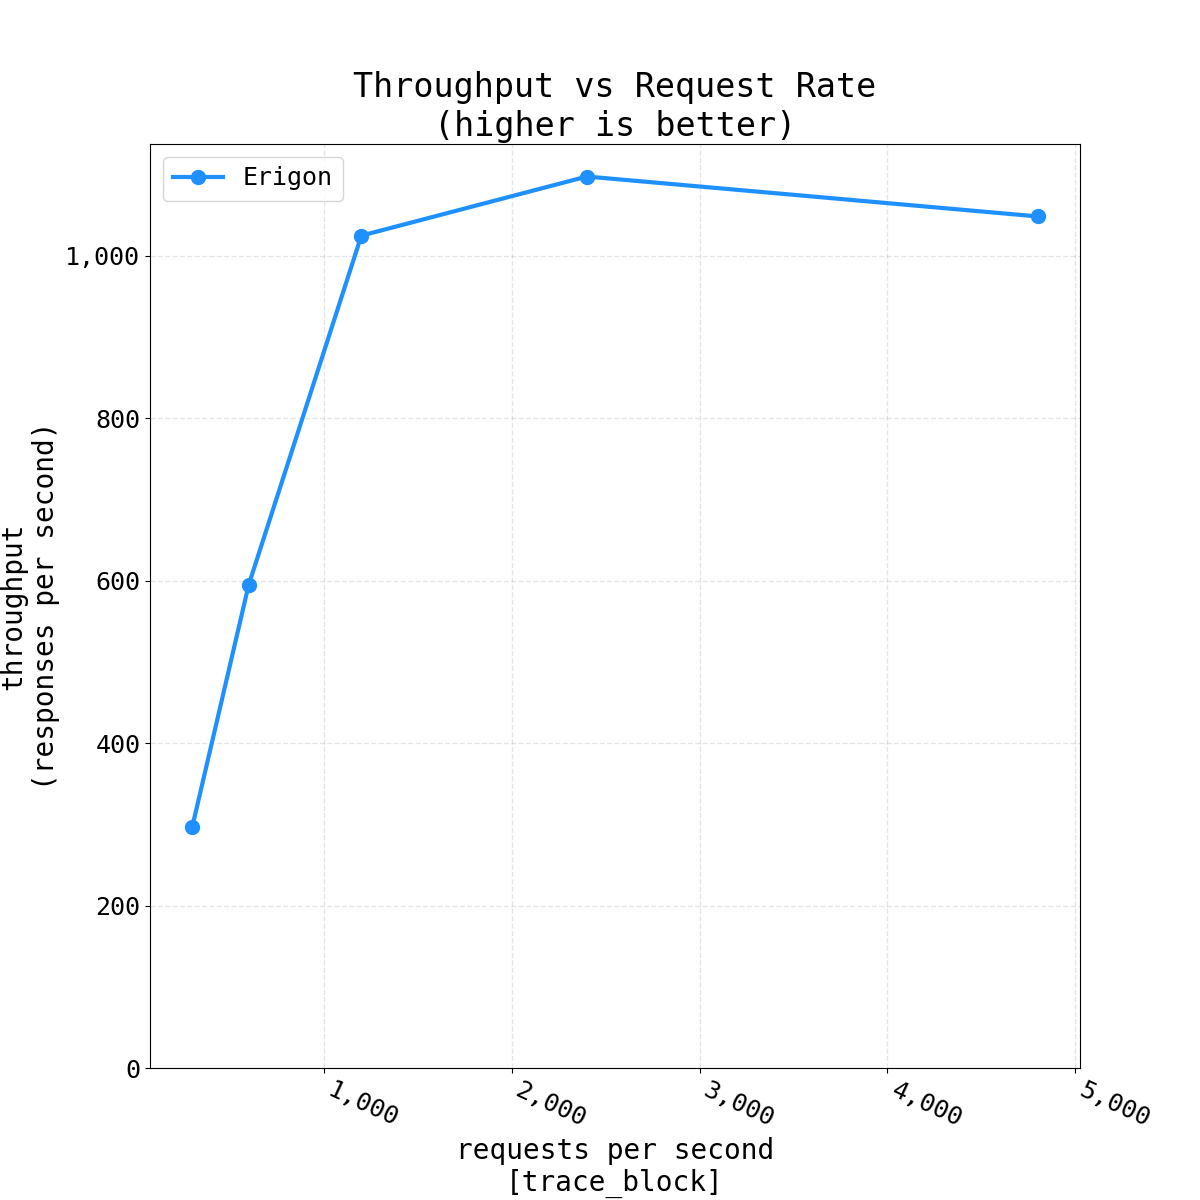
\includegraphics[width=0.7\textwidth]{Figures/results/load_tests/traces/throughput_trace.png}
    \caption{Throughput of {\tt trace\_block}. It reaches the maximum of around 1200 responses/s at 2400 requests/s. }
    \label{fig:traces-throughput}
\end{figure}

\begin{comment}

\begin{figure}[H]
    \centering
    \subfigure[]{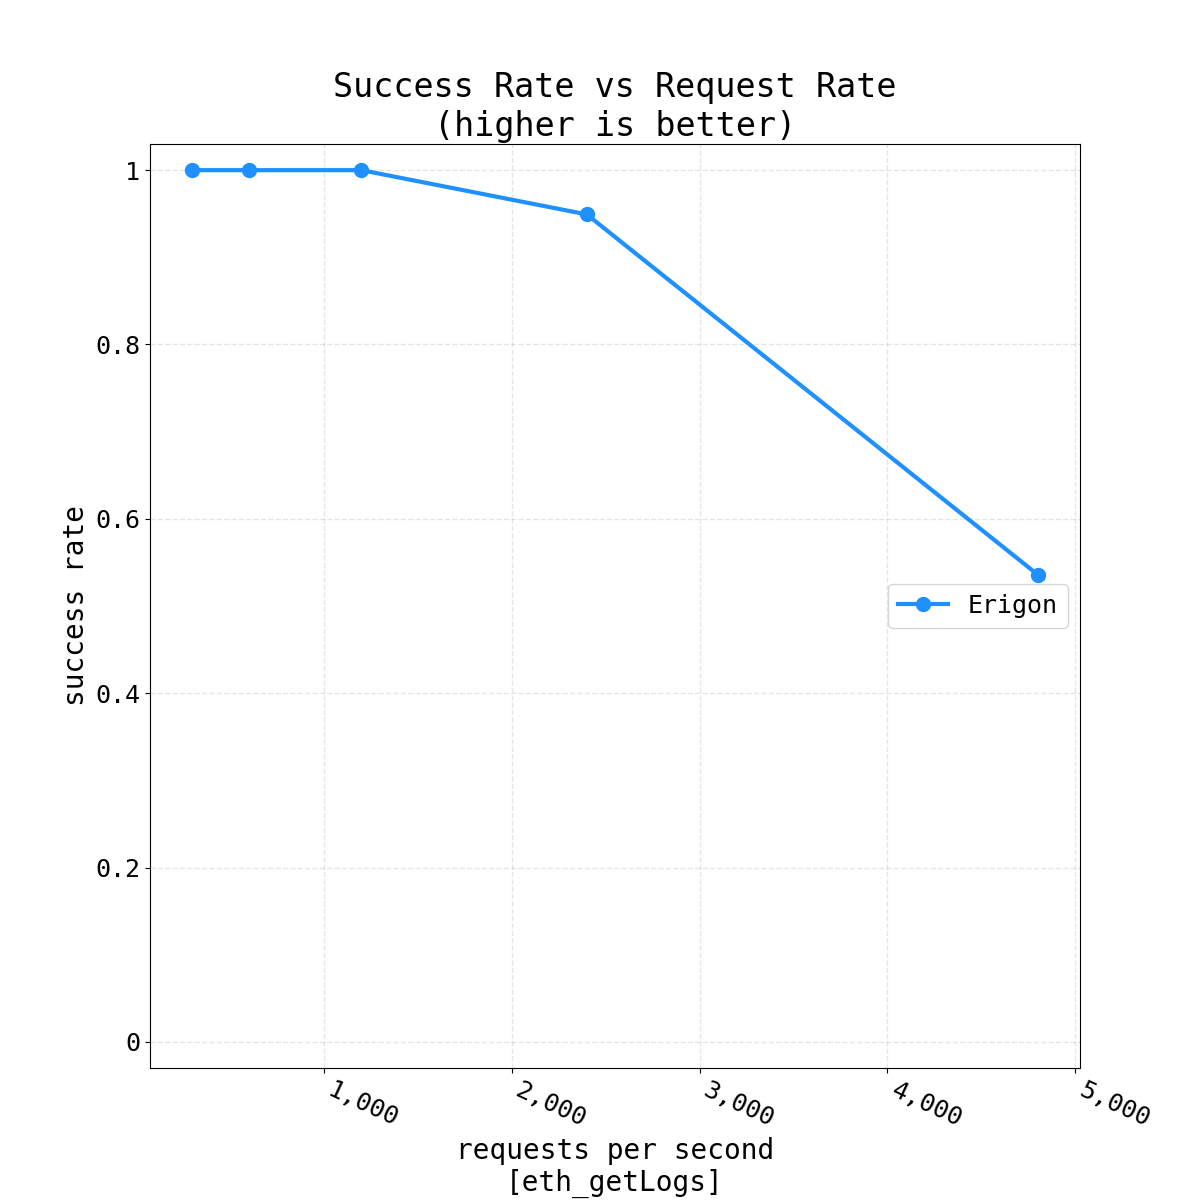
\includegraphics[width=0.48\textwidth]{Figures/results/load_tests/logs/success_rate_logs.png}} 
    \subfigure[]{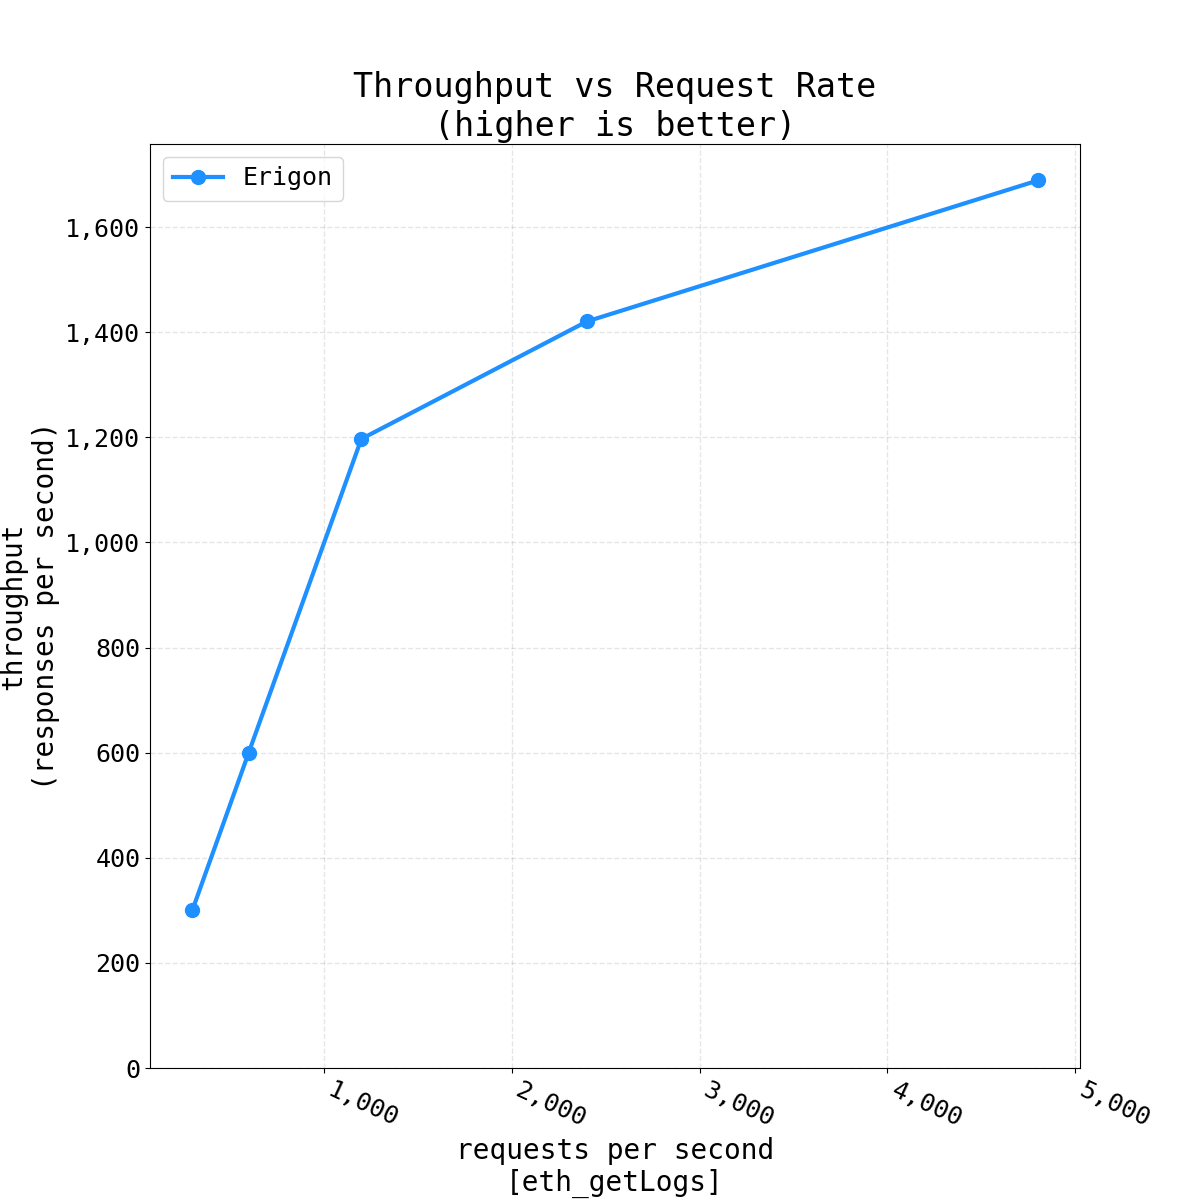
\includegraphics[width=0.48\textwidth]{Figures/results/load_tests/logs/throughput_logs.png}} 
    \subfigure[]{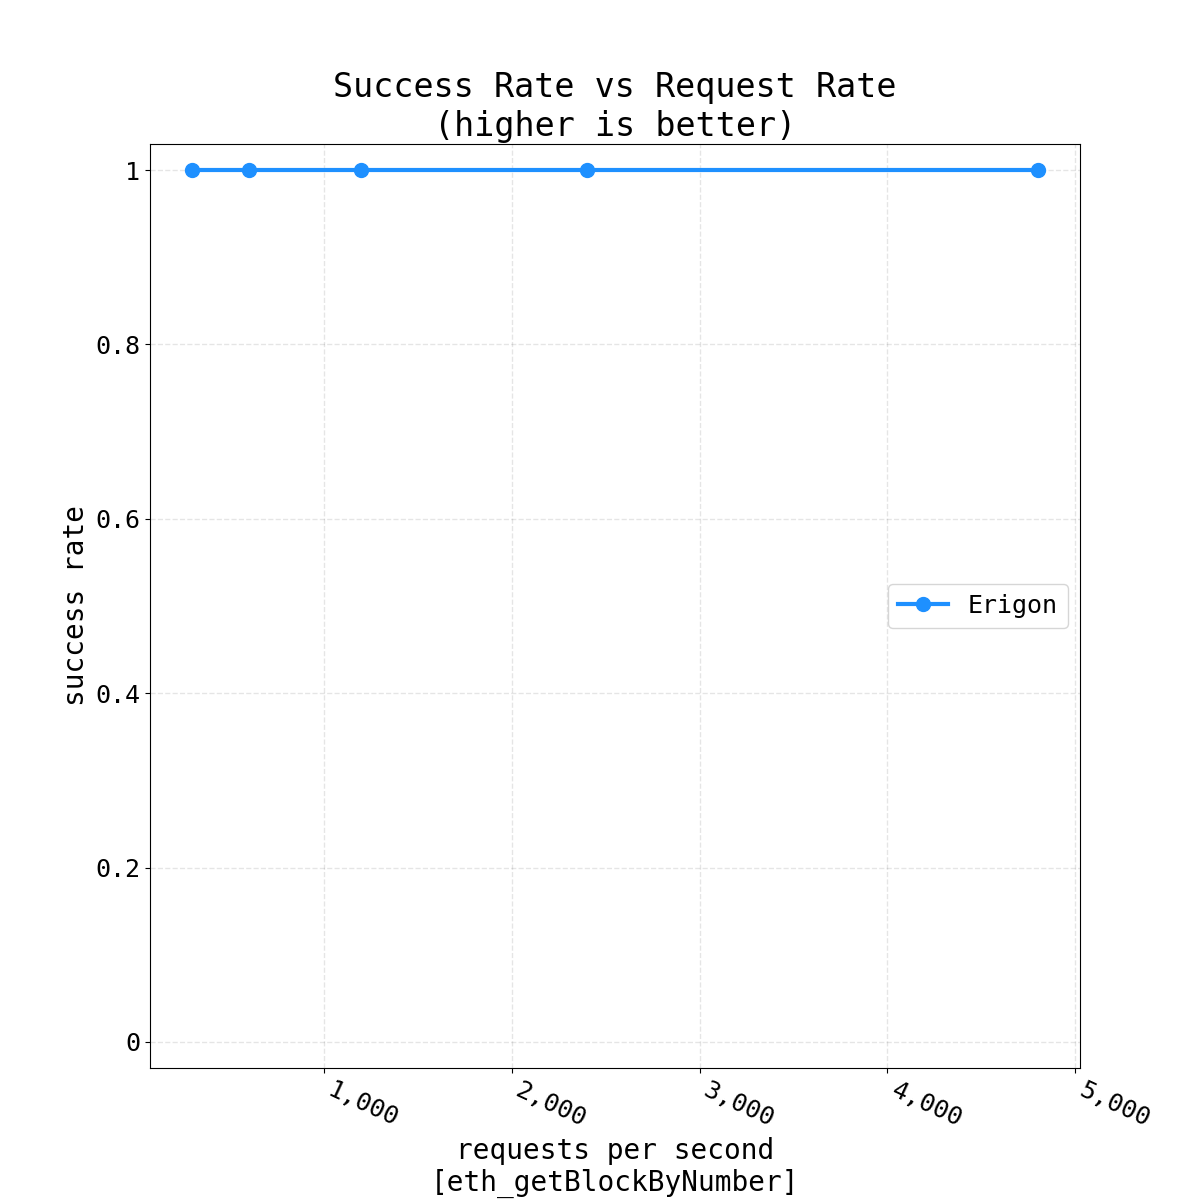
\includegraphics[width=0.48\textwidth]{Figures/results/load_tests/blocks/success_rate_blocks.png}}
    \subfigure[]{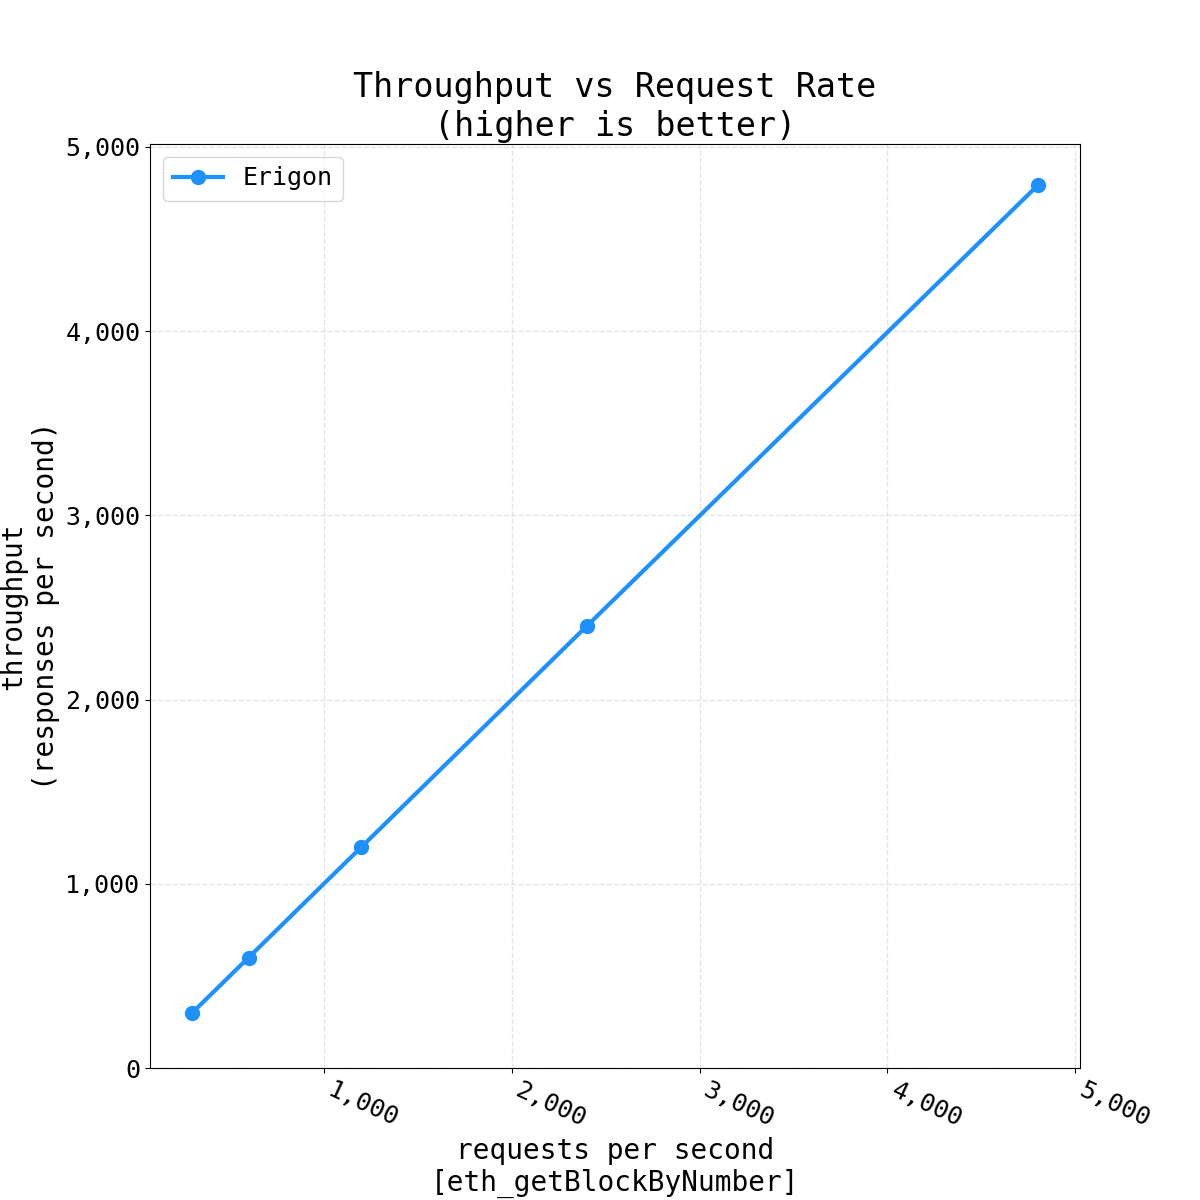
\includegraphics[width=0.48\textwidth]{Figures/results/load_tests/blocks/throughput_blocks.png}}
    \subfigure[]{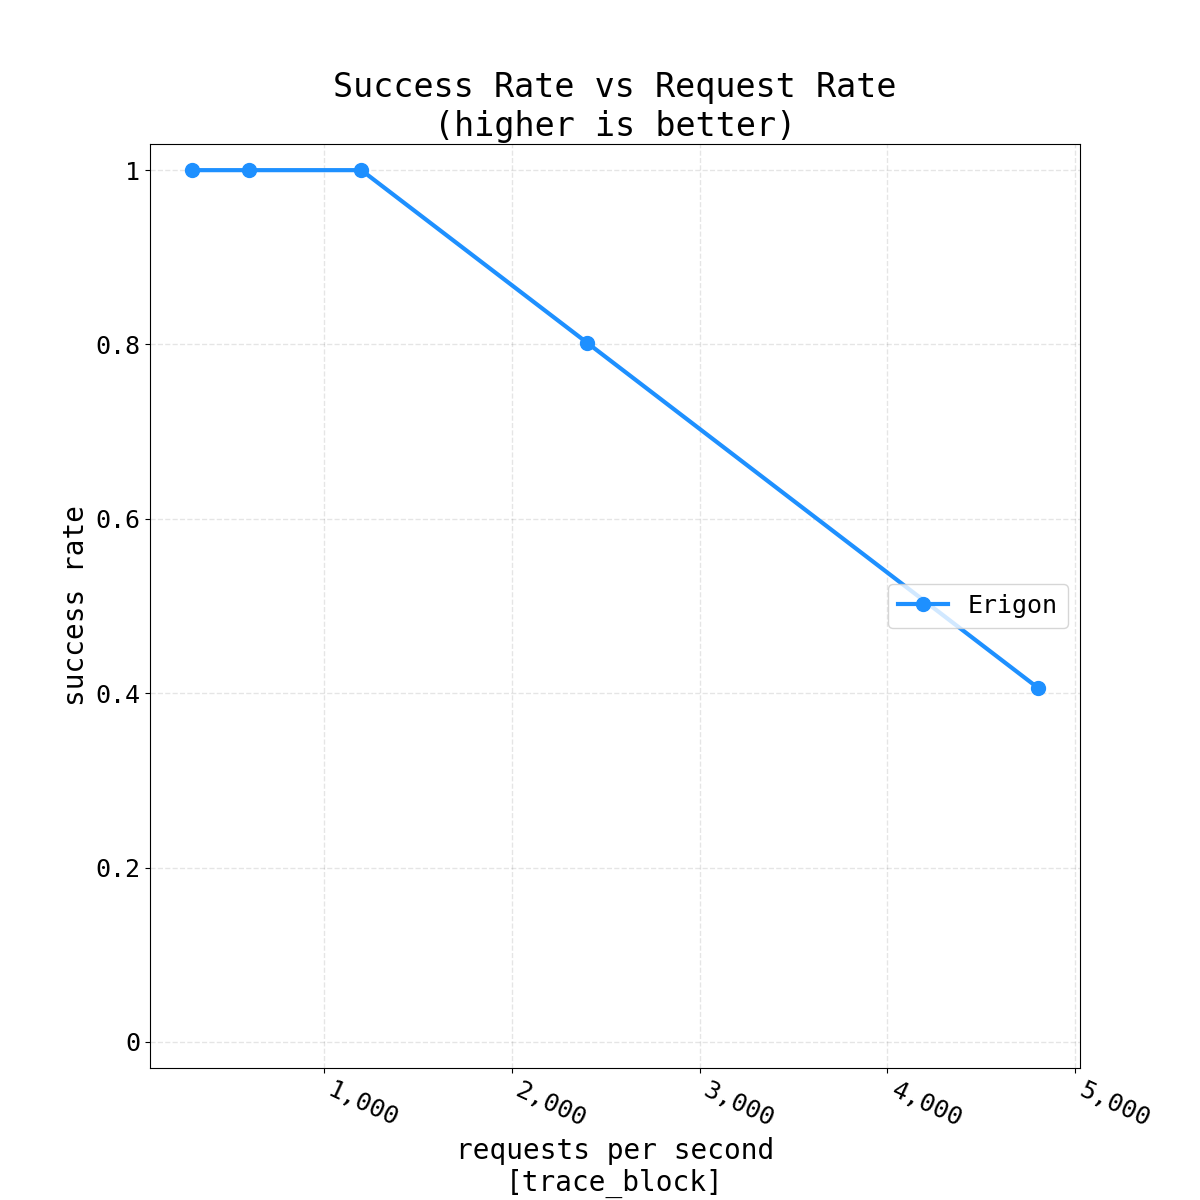
\includegraphics[width=0.48\textwidth]{Figures/results/load_tests/traces/success_rate_trace.png}}
    \subfigure[]{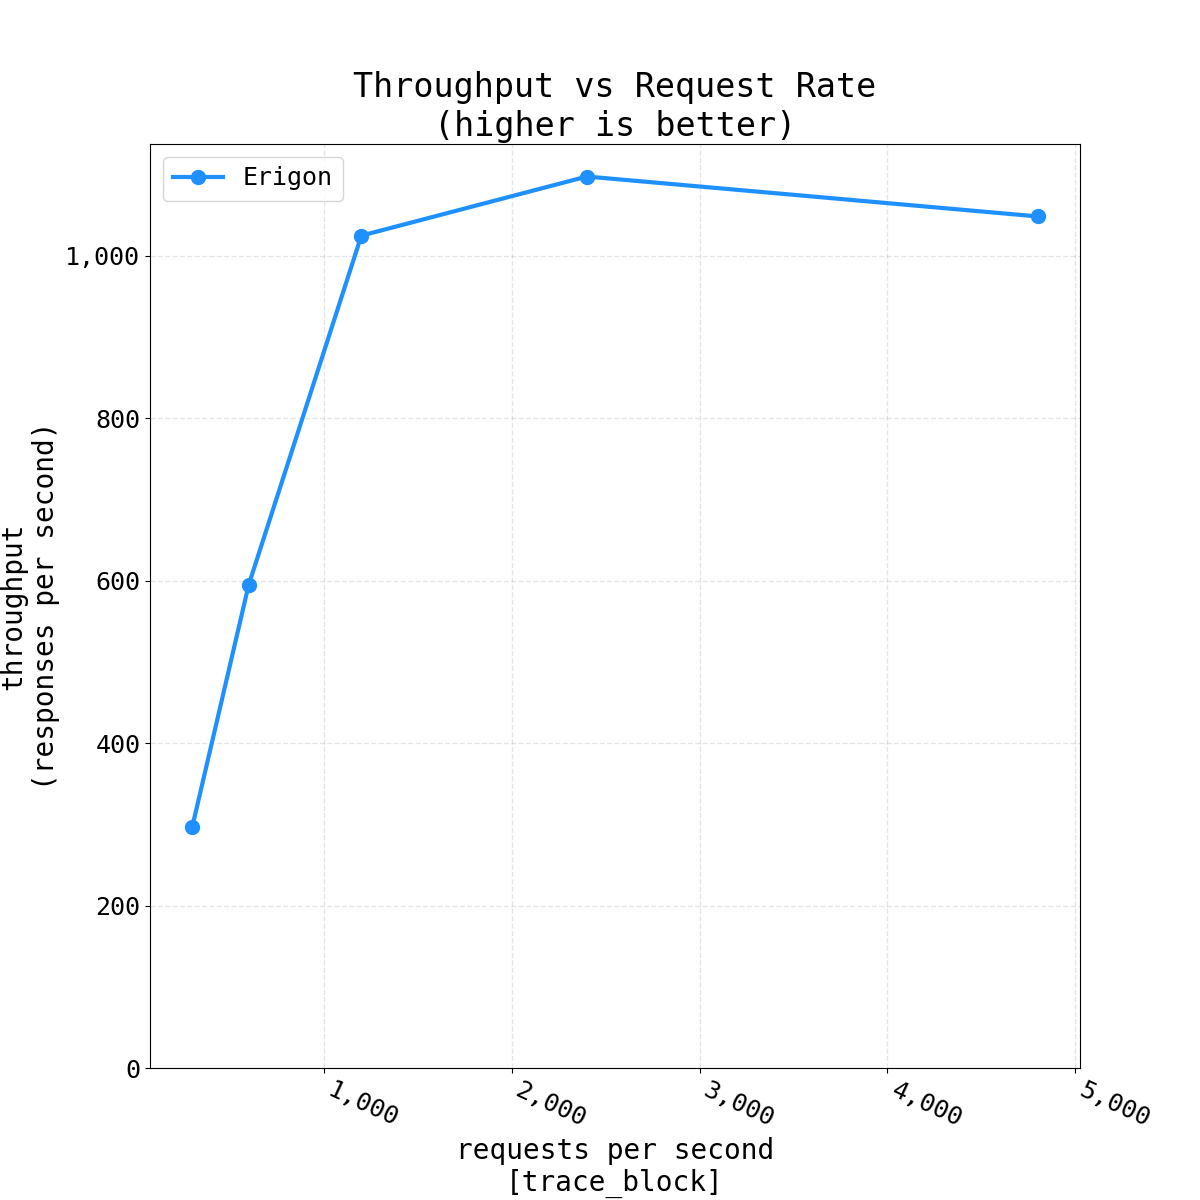
\includegraphics[width=0.48\textwidth]{Figures/results/load_tests/traces/throughput_trace.png}}
    \caption{Results of the load test for {\tt eth\_getLogs} (a, b), {\tt eth\_getBlockByNumber} (c, d) and {\tt trace\_block} (e, f).}
    \label{fig:load-test-results}
\end{figure}
    
\end{comment}


\section{Optimal number of concurrent tasks} 

\begin{figure}[!ht]
    \centering
    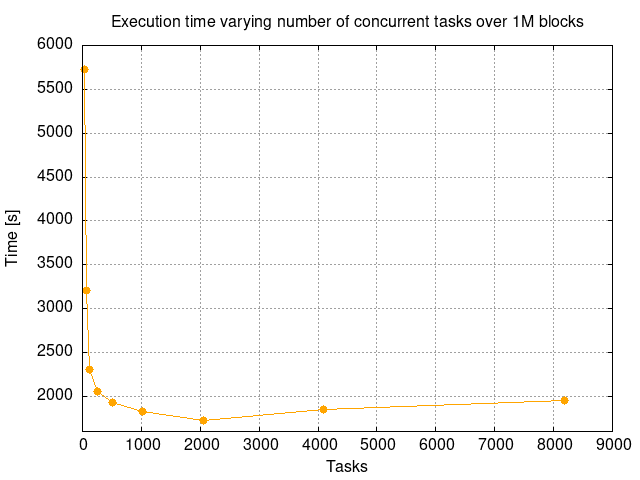
\includegraphics[width=0.8\textwidth]{Figures/results/num-tasks.png}
    \caption{Extraction time varying the number of concurrent tasks.}
    \label{fig:num-tasks}
\end{figure}

Eth2dgraph can be run with a variable amount of concurrent tasks that perform data extraction. This value can be set with the {\tt --num-tasks} option. Having too many concurrent tasks can overload the system where eth2dgraph is ran or the Ethereum node used, while having just few tasks make the extraction process very slow.

To find a good value for the number of tasks, I ran eth2dgraph with different amount of tasks over one million blocks, from 10M to 11M. \cref{fig:num-tasks} shows the results of this test. As observed from the data, the optimal number of tasks for the machine used is around 2048, that is eight times the amount of available threads.

\section{Extraction of data}

\subsection{Extraction and Transformation}

To perform the extraction and transformation of Ethereum data to Dgraph format, eth2dgraph was run with the command reported in \cref{lst:extract-command}. The extraction was performed from block $0$ to block $17,265,420$, using $2048$ concurrent tasks. 

\begin{lstlisting}[language=Bash,caption={Eth2dgraph extraction command used.},label={lst:extract-command},captionpos=b,numbers=none]
eth2dgraph extract \
    -o extraction_output \
    -f 0 \
    -t 17265420 \
    --num-tasks 2048 \
    --include-tx \
    --include-transfers \
    --include-logs \
    -s smart-contract-sanctuary-ethereum/ \
    --size-output 100000 > eth2dgraph_extraction.logs & disown
\end{lstlisting}

\cref{table:extraction-stats} reports general statistics about the extraction process. The detailed sizes of the output folders are reported in \cref{table:extraction-output}.

\cref{fig:ram-usage-extraction} and \cref{fig:cpu-usage-extraction} shows respectively the RAM and CPU usage of the server during the process of data extraction. Data was obtained using the command~{\tt top -bn1 | awk '/Cpu/ \{ print \$2 \}' }~for the CPU and~{\tt free -m | awk '/Mem/\{print \$3\}' }~for the memory.
  

\begin{table}[H]
\centering
    \begin{threeparttable}
    \begin{tabular}{ m{5cm} m{3cm} } 
    \toprule
    \textbf{Parameter} & \textbf{Value}\\
    \midrule
    Total time   & 7h 15m 21s   \\ [1.2ex]
    Block/s      & 660.97       \\ [1.2ex]
    Contracts    & 60,016,663   \\ [1.2ex]
    Contract/s   & 2,297.6       \\ [1.2ex]
    Decompiler failures & 508,990 \\ [1.2ex]
    Output size  & 957 GiB        \\ [1.2ex]
    \bottomrule
    \end{tabular}
    \end{threeparttable}
    \caption{Statistics about extraction and transformation process.}
    \label{table:extraction-stats}
\end{table}

\begin{table}[H]
\centering
    \begin{threeparttable}
    \begin{tabular}{ m{5cm} m{3cm} } 
    \toprule
    \textbf{Folder} & \textbf{Size}\\
    \midrule
    {\tt / } & 957GiB \\
    {\tt /dynamic }    & 934GiB \\
    {\tt /static }     & 24GiB  \\
    & \\
    {\tt /static/blocks } & 1.2GiB  \\
    {\tt /static/events } & 548KiB    \\
    {\tt /static/destructions } & 3.4GiB    \\
    {\tt /static/deployments } & 18GiB  \\    
    {\tt /static/skeletons } & 903MiB    \\
    {\tt /static/errors } & 36KiB     \\
    {\tt /static/functions } & 8.5MB  \\  
    & \\
    {\tt /dynamic/transfers } & 129GiB    \\
    {\tt /dynamic/logs } & 263GiB    \\
    {\tt /dynamic/transactions } & 543GiB    \\
    \bottomrule
    \end{tabular}
    \end{threeparttable}
    \caption{Size of extracted data divided by folders.}
    \label{table:extraction-output}
\end{table}

\begin{figure}[H]
    \centering
    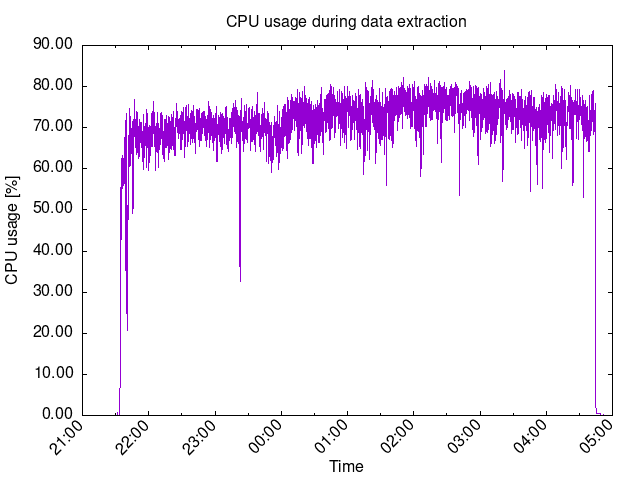
\includegraphics[width=0.9\textwidth]{Figures/results/cpu-usage-extraction.png}
    \caption{CPU usage of the server during data extraction.}
    \label{fig:cpu-usage-extraction}
\end{figure}

\begin{figure}[H]
    \centering
    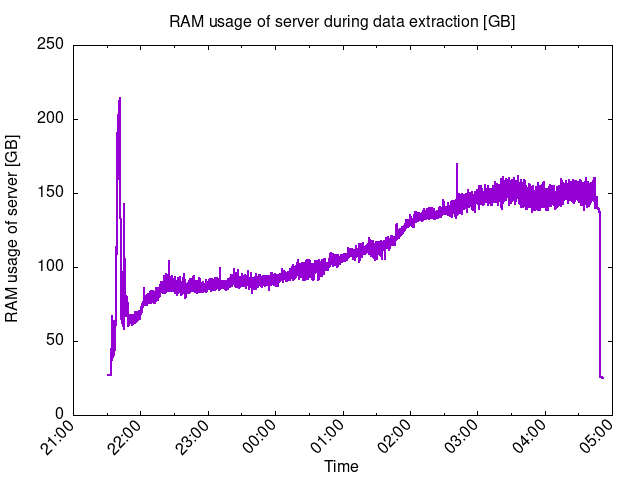
\includegraphics[width=0.9\textwidth]{Figures/results/ram-usage-extraction.png}
    \caption{Memory used by the server during data extraction}
    \label{fig:ram-usage-extraction}
\end{figure}

\subsection{Import in Dgraph}

Data was imported in Dgraph using the Bulk Loader. I faced a problem during the import of the complete dataset, the loader kept crashing. Analyzing the logs, it seemed that the crash was due to a hard limit on the size of local buffers. Removing this hard-coded limit allowed me to complete the import of data. I also submitted this fix\footnote{Pull Request can be seen here: \url{https://github.com/dgraph-io/dgraph/pull/8841}} in the open-source codebase of Dgraph. It was accepted, merged in the main branch and later included in the 23.0.1 release.

To perform the bulk import, I first ran with \cref{lst:zero-command} an instance of {\tt zero}, the Dgraph's node responsible of coordinating the distributed cluster. With the {\tt zero} running, the bulk import process was started with command reported in \cref{lst:bulk-command}.

\begin{lstlisting}[language=Bash,caption={Command used for running {\tt zero}.},label={lst:zero-command},captionpos=b,numbers=none]
    dgraph zero --my=localhost:5080
\end{lstlisting}

\begin{lstlisting}[language=Bash,caption={Command used for running {\tt bulk loader}.},label={lst:bulk-command},captionpos=b,numbers=none]
dgraph bulk -f "<data-location>" \
	-s "<dql-schema-location>" \
	-g "<graphql-schema-location>" \
	--out "./out" \
	--map_shards=4 \
	--reduce_shards=1 \
	--zero=localhost:5080 \
	--mapoutput_mb=4096 \
	--num_go_routines=64 \
  --cleanup_tmp=false
\end{lstlisting}

The import of the complete dataset took 52 hours. Divided in 28 hours for the MAP phase and 24 hours for the REDUCE phase. It resulted to be the bottleneck of all the process, it took around 7.5 times the amount of time needed for extracting the data. 

For memory heavy operations, Dgraph does not rely on the Go garbage collector, it uses \textit{jemalloc} to manually allocate memory. \cref{fig:import-ram-usage,fig:import-cpu-usage} show the RAM allocated by Dgraph during the phases of MAP and REDUCE of the bulk import. At least 400GiB of RAM are needed. Both steps have shown a big spike in memory allocation at around half of the process. The reasons of these spikes are not clear.

\begin{figure}[H]
    \centering
    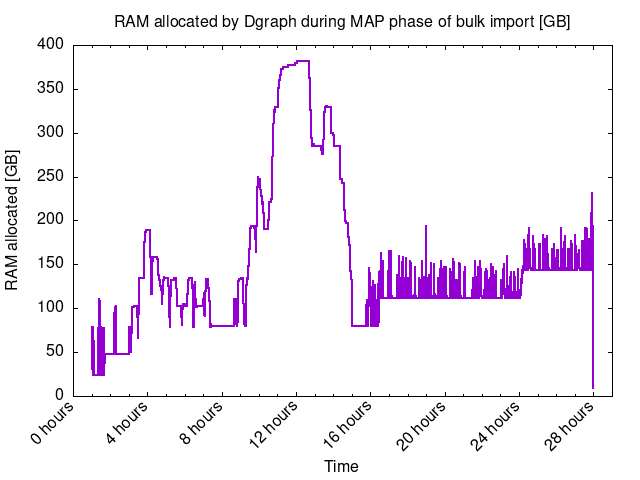
\includegraphics[width=0.9\textwidth]{Figures/results/MAP_RAM.png}
    \caption{RAM allocated by Dgraph with jemalloc during the MAP phase of the bulk import.}
    \label{fig:import-ram-usage}
\end{figure}

\begin{figure}[H]
    \centering
    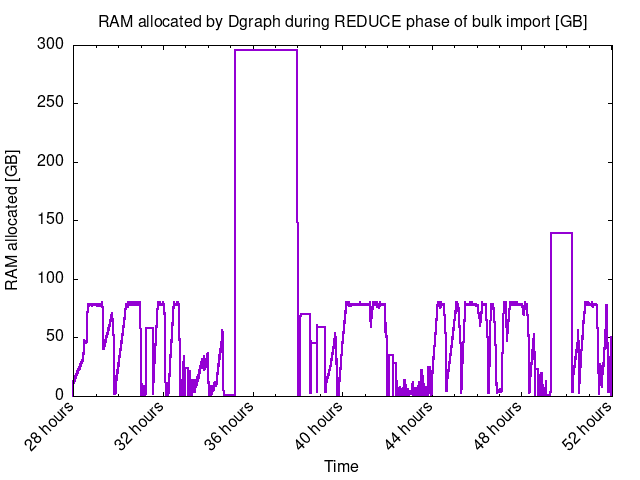
\includegraphics[width=0.9\textwidth]{Figures/results/REDUCE_RAM.png}
    \caption{RAM allocated by Dgraph with jemalloc during the REDUCE phase of the bulk import.}
    \label{fig:import-cpu-usage}
\end{figure}

The result of the bulk import is a folder called~{\tt p}~that contains the actual data in Dgraph's binary format. The size of this folder was of 2.5 TiB. 

From this folder, {\tt alpha}, the node responsible for managing the actual data, was run with the command shown in \cref{lst:alpha-command}. All the process was done with a locally-compiled version of Dgraph, but it is possible to perform the same steps using Docker. The details of the imported data, divided by types, are reported in \cref{table:imported-data-sizes}.

In contrast to importing the entire dataset, the import of the static data alone was completed in 1 hour, with an output of 112 GiB. This smaller dataset statically describes all the smart contracts of the Ethereum blockchain, without information on their usage. 

\begin{lstlisting}[language=Bash,caption={Command used for running the {\tt alpha} instance.},label={lst:alpha-command},captionpos=b,numbers=none]
dgraph alpha 
    --my=localhost:7080 \
    --zero=localhost:5080 \
    --security whitelist=0.0.0.0/0 \
    --cache "size-mb=20000; percentage=50,30,20;" \
    --badger="compression=snappy; numgoroutines=64;"
\end{lstlisting}

\begin{table}[H]
\centering
    \begin{threeparttable}
    \begin{tabular}{ m{3.8cm} m{3cm} m{2cm} m{4cm} } 
    \toprule
    \textbf{Type} & \textbf{Entries} & \textbf{Disk size} & \textbf{Uncompressed size} \\
    \midrule
    Transaction   & 1,967,716,025 & 1.3TiB & 2.8TiB \\ [1.2ex]
    Log   & 2,795,971,346 & 823.6GiB & 2.2TiB \\ [1.2ex]
    TokenTransfer   & 1,437,470,051 & 181.1GiB & 414.0GiB \\ [1.2ex]
    ContractDeployment   & 60,016,663 & 82.0GiB & 161.3GiB \\ [1.2ex]
    Account   & 286,391,265 & 29.7GiB & 52.2GiB \\ [1.2ex]
    ContractDestruction   & 55,152,100 & 9.7GiB & 22.5GiB \\ [1.2ex]
    Block   & 17,265,421 & 5.7GiB & 16.7GiB \\ [1.2ex]
    Skeleton   & 467,318 & 1.5GiB & 7.0GiB \\ [1.2ex]
    Withdrawal   & 3,688,662 & 285.7MiB & 956.5MiB \\ [1.2ex]
    Function   & 139,603 & 42.1MiB & 84.9MiB \\ [1.2ex]
    Event   & 9,690 & 2.1MiB & 4.0MiB \\ [1.2ex]
    Error   & 545 & 118.5KiB & 228.6KiB \\ [1.2ex]
    \bottomrule
    \end{tabular}
    \end{threeparttable}
    \caption{Cardinalities and sizes of entries stored in Dgraph\protect\footnotemark.}
    \label{table:imported-data-sizes}
\end{table}
\footnotetext{Data about sizes was obtained querying the {\tt /state} endpoint of the {\tt alpha} instance.}

 \section{Querying data}

Dgraph exposes two endpoints for querying the data: one for DQL at \\{\tt /query} and one for GraphQL at {\tt /graphql}.

DQL is the query language built by the Dgraph team to query and mutate data in this database. It has powerful features such as query variables, math on attributes, recursive queries and shortest path search. Under the hood, every GraphQL query is translated to DQL before being executed, so everything that can be done with GraphQL can be done with DQL, but not the opposite.

To easily perform DQL queries, Dgraph provides a web application called \textit{Ratel}\footnote{Ratel is a web application for querying, visualizing and managing Dgraph's data: \url{https://github.com/dgraph-io/ratel}}. It gives a friendly user interface to get and visualize query results. \cref{fig:ratel-1} shows an example of query in which it is visualized the ABI of a contract. \cref{fig:ratel-2} shows accounts linked by transactions.

\begin{figure}[H]
    \centering
    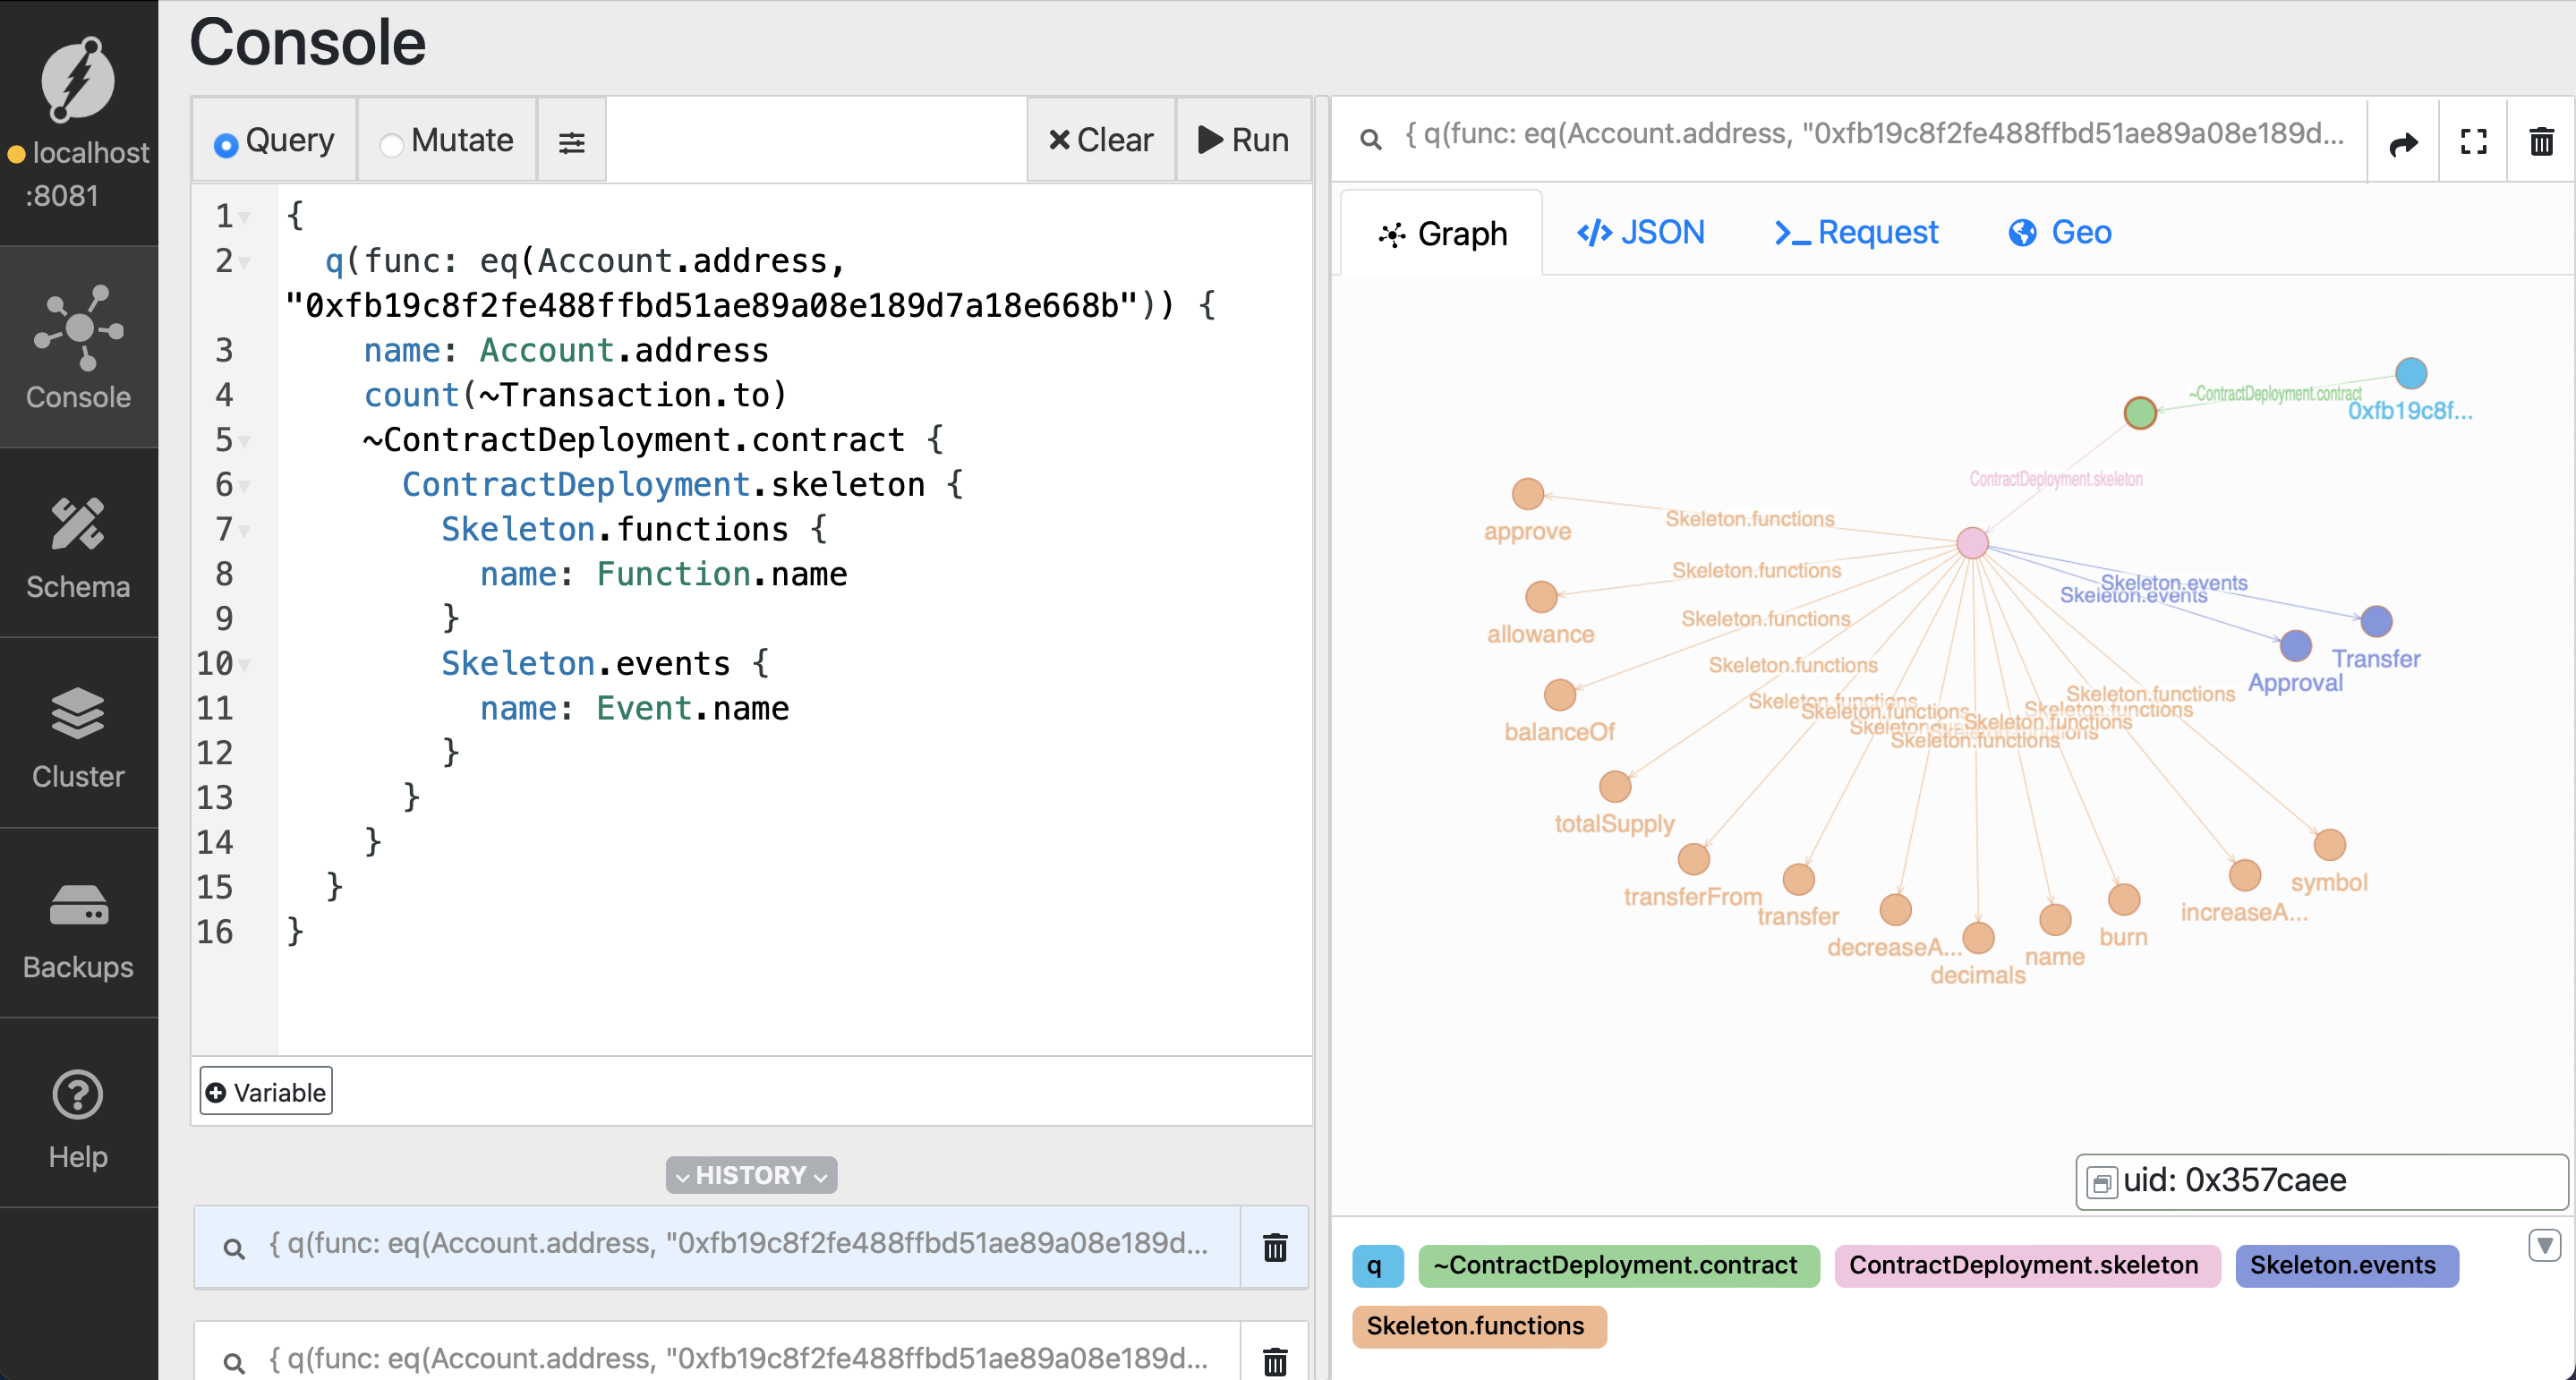
\includegraphics[width=1\textwidth]{Figures/results/ratel-1.png}
    \caption{Visualization of Contract's ABI in Ratel.}
    \label{fig:ratel-1}
\end{figure}

\begin{figure}[H]
    \centering
    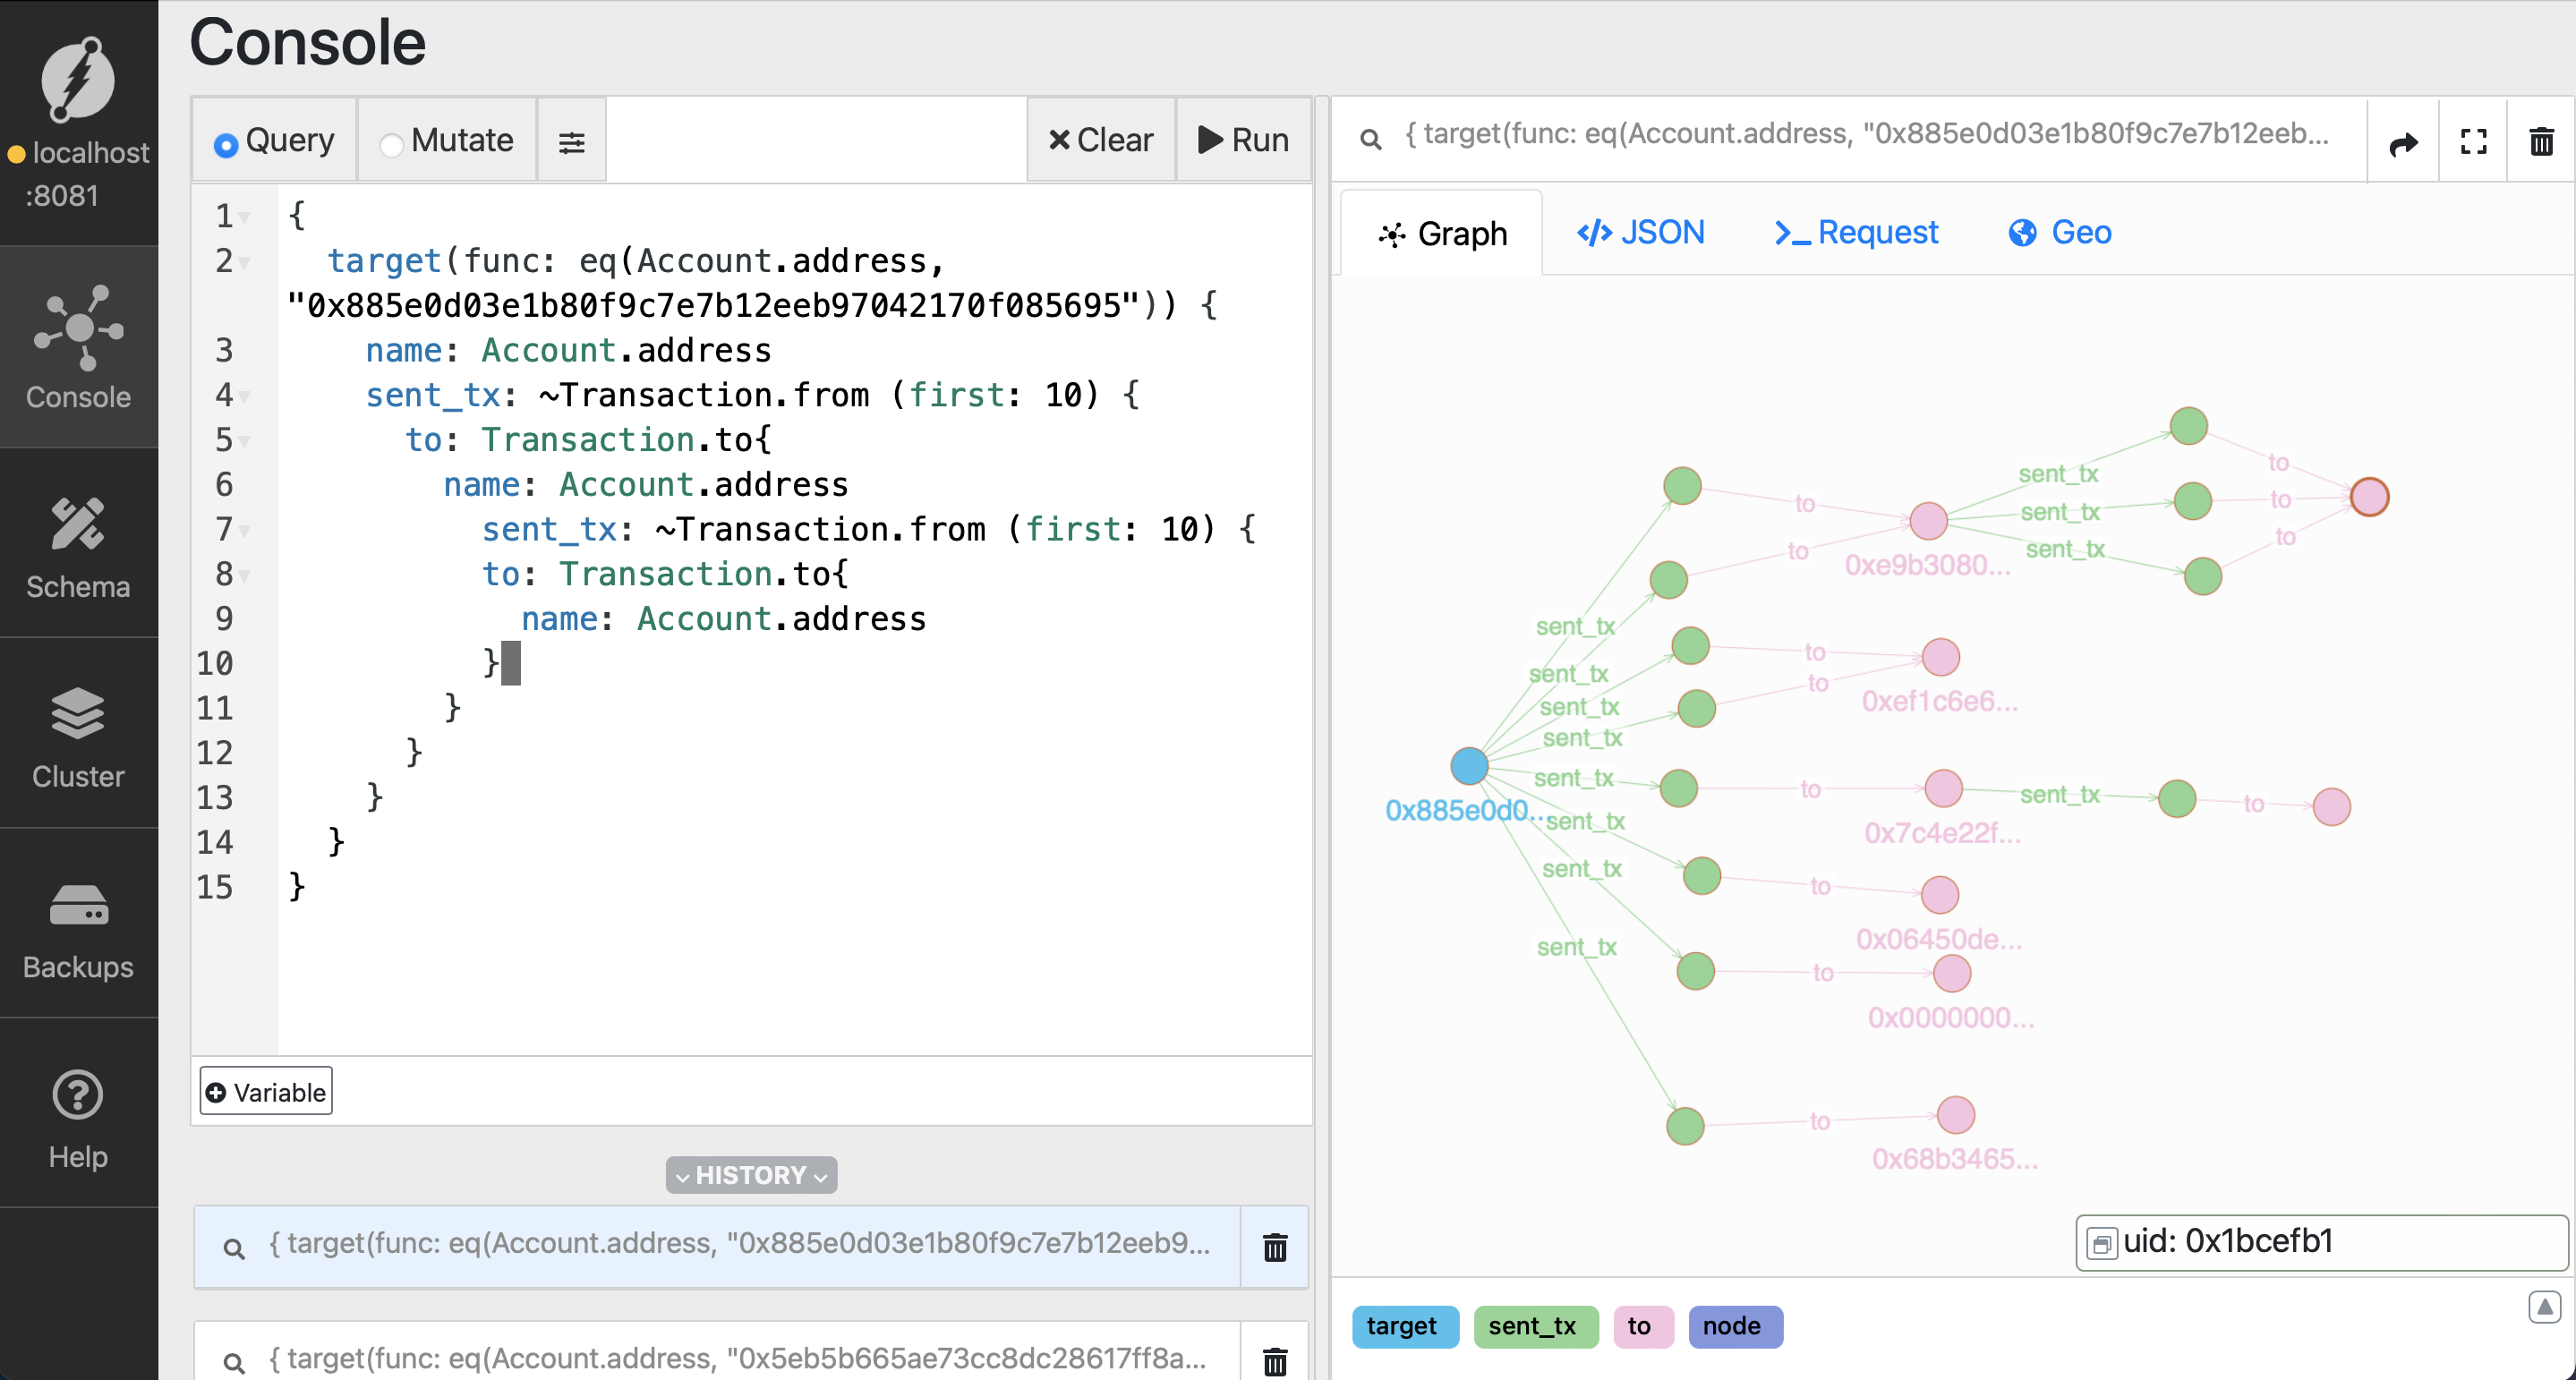
\includegraphics[width=1\textwidth]{Figures/results/ratel-2.png}
    \caption{Visualization of Accounts linked by Transactions in Ratel.}
    \label{fig:ratel-2}
\end{figure}

\subsection{Query performance}

In this section, I provide examples of queries with their corresponding execution times. The processing time mentioned in table \cref{table:queries-results} is included by the database in the query responses. It does not include decoding, encoding or network transfers, just the time needed by Dgraph to get the data.

\begin{lstlisting}[caption={Query to get all the transactions sent by a specific address. Response included 1071 transactions.},label={lst:query-1},captionpos=b,numbers=none]
{
    q(func: eq(Account.address, "0xd8da6bf26964af9d7eed9e03e53415d37aa96045")){
        ~Transaction.from{
            expand(_all_)
        }
    }
}
\end{lstlisting}

\begin{lstlisting}[caption={Query to get all the transfers of BoredApe NFT with id \textit{1020} (686 transfers).},label={lst:query-2},captionpos=b,numbers=none]
{
    BOREDAPE as var(func: eq(Account.address, "0xbc4ca0eda7647a8ab7c2061c2e118a18a936f13d"))
	q(func: uid(BOREDAPE)) {
        transfers: ~TokenTransfer.contract @filter(eq(TokenTransfer.token_id, "1020" )) {
            TokenTransfer.block {
                Block.number
                Block.datetime
            }
            TokenTransfer.from {
                Account.address
            }
            TokenTransfer.to {
                Account.address
            }
        }
	}
}
\end{lstlisting}

\begin{lstlisting}[caption={Query to count all the transactions in the database.},label={lst:query-3},captionpos=b,numbers=none]
{
    var(func: type(Transaction)) {
        countVar as count(uid)
    }
    agg() {
        count: max(val(countVar))
    }
}
\end{lstlisting}

\begin{lstlisting}[caption={Query to get the addresses of contracts that implement a function with name \textit{trade} (554 addresses).},label={lst:query-4},captionpos=b,numbers=none]
{
    q(func: eq(Function.name, "trade")) @normalize {
        ~Skeleton.functions {
            ~ContractDeployment.skeleton {
                ContractDeployment.contract {
                    address: Account.address
                }
            }
        }
    }
}
\end{lstlisting}

\begin{lstlisting}[caption={Query to compute the ETH burnt after London upgrade.},label={lst:query-5},captionpos=b,numbers=none]
{
    var(func: ge(Block.number, 12965000))  {
        price as Block.base_fee_per_gas
        used as Block.gas_used
        gasBurnt as math(price * used)
    }
    q() {
        totBurnt as sum(val(gasBurnt))
        ethBurnt as math(totBurnt / 1000000000)
        usdBurnt: math(ethBurnt * 1870) 
    }
}
\end{lstlisting}

\begin{table}[H]
\centering
    \begin{threeparttable}
    \begin{tabular}{ m{3cm} m{5cm} } 
    \toprule
    \textbf{Query} & \textbf{Processing time [ms]}\\
    \midrule
    \cref{lst:query-1}   & 1671.46  \\ [1.2ex]
    \cref{lst:query-2}   & 416.70  \\ [1.2ex]
    \cref{lst:query-3}   & 73881.76  \\ [1.2ex]
    \cref{lst:query-4}   & 165.65  \\ [1.2ex]
    \cref{lst:query-5}   & 31868.36  \\ [1.2ex]
    \bottomrule
    \end{tabular}
    \end{threeparttable}
    \caption{Processing time of DQL queries. }
    \label{table:queries-results}
\end{table}
 
\section{Comparison with Ethereum-ETL}

Eth2dgraph was compared against Ethereum-ETL, one of the most popular open source tool to export Ethereum data. The two tools serve the same purpose: extract and transform Ethereum data to be more usable.
Ethereum-ETL does so exporting data to CSV files, that can eventually be loaded into relational databases, while eth2dgraph does so exporting data to compressed JSON files that can be imported into Dgraph. 

At high level, the two tools work in a similar way. They both fetch data using the Ethereum RPC interface. They both can be used trough a CLI.

Ethereum-ETL does not integrate a decompiler to get the ABI of the smart contracts. It simply stores the raw four bytes of the function selectors that can be found as arguments of the {\tt PUSH4} opcode in the beginning of the contracts' bytecodes. 

Another design difference is in the steps needed to get the data. Ethereum-ETL needs multiple extraction steps to get certain kind of information. For example, to get smart contracts data, it first needs to get and store the list of contracts' addresses, then, for each address, if fetches the contract's data. Eth2dgraph does everything in a single extraction step using the traces, to make the process faster.

The comparison was made by extracting data on various block ranges. There are multiple ways of using Ethereum-ETL. For this comparison it was run with the command {\tt export\_all}. This command produces a similar output to the one of eth2dgraph, with the difference that it includes transaction receipts but it does not use the traces. The usage of receipts instead of traces means that all the contracts created by other contracts are not included in the output data. 

\cref{lst:ethereum-etl-command,lst:eth2dgraph-command} show the commands used to run the tools for the comparison. Both tools were run in the same machine and using the same Ethereum node. For the run on 400k blocks, Ethereum-ETL was run with batch size\footnote{The batch size indicates how many calls are sent together to the Ethereum node.} reduced to 20. This was done since the default size of 100 caused the program to crash. The results are reported in \cref{table:tools-comparison-2}. 

\begin{lstlisting}[caption={Command for running Ethereum-ETL in the comparison},label={lst:ethereum-etl-command},captionpos=b,numbers=none]
ethereumetl export_all \
    -s <from> \
    -e <to> \
    -p http://localhost:8545 \
    -o <output-folder> \
    -w 2048
\end{lstlisting}

\begin{lstlisting}[caption={Command for running eth2dgraph in the comparison},label={lst:eth2dgraph-command},captionpos=b,numbers=none]
eth2dgraph extract \
    -f <from> \
    -t <to> \
    --num-tasks 2048 \
    --include-tx \
    --include-logs \
    --include-transfers \
     -o <output-folder> 
\end{lstlisting}

\begin{table}[H]
\centering
    \begin{threeparttable}
    \begin{tabular}{ c c c c } 
    \toprule
    \textbf{Blocks range} & \textbf{Ethereum-ETL} & \textbf{eth2dgraph} & \textbf{Speedup} \\
    \midrule
    12000000-12001000   & 1m 57s & 8s & 14.6x \\ [1.2ex]  
    16000000-16010000   & 14m 18s & 53.48s & 16x \\ [1.2ex] 
    17000000-17100000   & 2h 56m 53s & 6m 45s & 26.2x \\ [1.2ex]   
    14000000-14400000   & 13h 30m 21s & 31m 10s & 48x \\ [1.2ex]
    \bottomrule
    \end{tabular}
    \end{threeparttable}
    \caption{Results of performance comparison between Ethereum-ETL and eth2dgraph. }
    \label{table:tools-comparison-2}
\end{table}

Overall, eth2dgraph was at least one order of magnitude faster than Ethereum-ETL in all the extractions performed. This shows the effectiveness of the design choices taken while developing eth2dgraph. With growing block ranges, eth2dgraph becomes faster because the caching logic allows it to avoid decompiling contracts.

